%%%%%%%%%%%%%%%%%%
%%%   Template para utilização   %%%
%%%%%%%%%%%%%%%%%%

%Para melhor utilização da ferramenta, utilize o pdfLaTeX+MakeIndex+BibTeX%

\documentclass[12pt,openright,oneside,a4paper,english,french,spanish,brazil]{unifil}

\usepackage{abntex2cite}

\titulo{Objeto de Aprendizado - Simulador MRI} %Atualizar conforme progredir%
\autor{Rodrigo de Souza Castoldi}
\instituicao{Centro Universitário Filadélfia}
\local{Londrina}
\data{2017}
\preambulo{Ciência da Computação}
\orientador{Prof. Me. Ricardo Inácio Álvares e Silva}

\begin{document}

\frenchspacing

%%%%%%%%%%%%%%%%%%%%%%%%%
%%%%%%Elementos pré-textuais%%%%%%%%%
%%%%%%%%%%%%%%%%%%%%%%%%%

\pretextual

%Capa%

\imprimircapa

%Folha de Rosto%

\makeatletter
\renewcommand{\folhaderostocontent}{
\begin{center}
{\ABNTEXchapterfont\bfseries\MakeTextUppercase{\imprimirautor}}
\vspace*{5cm}
\begin{center}
\ABNTEXchapterfont\bfseries\normalsize\MakeTextUppercase{\imprimirtitulo}
\end{center}
\vspace*{1cm}
\abntex@ifnotempty{\imprimirpreambulo}{%
\hspace{.45\textwidth}
\begin{minipage}{.5\textwidth}
\SingleSpacing
Trabalho de Dissertação apresentado ao \imprimirinstituicao{} como parte dos requisitos para obtenção de graduação em \imprimirpreambulo.
{\textnormal{\imprimirorientadorRotulo~\imprimirorientador.}}
\end{minipage}%
}%
\vspace*{\fill}
{\bfseries\large\imprimirlocal}
\par
{\bfseries\large\imprimirdata}
\vspace*{1cm}
\end{center}
}
\makeatother

\imprimirfolhaderosto

\clearpage{\pagestyle{empty}\cleardoublepage}

%Folha de Aprovação%

\begin{folhadeaprovacao}
	\begin{center}
		\ABNTEXchapterfont\textbf{\MakeTextUppercase{\imprimirautor}}
		\vspace*{2cm}
		\begin{center}
			\ABNTEXchapterfont\large\textbf{\MakeTextUppercase{\imprimirtitulo}}
		\end{center}
		\vspace*{2cm}
		Trabalho de Conclusão de Curso apresentado à Banca Examinadora do curso de \imprimirpreambulo{} do \imprimirinstituicao{} de \imprimirlocal{} em cumprimento a requisito parcial para obtenção do título de Bacharel em \imprimirpreambulo.
		\par
		\vspace*{.5in}
		\hspace{.6\textwidth}
		\begin{minipage}{.6\textwidth}
			\begin{center}
\MakeTextUppercase{Aprovado pela \textbf{COMISSÃO EXAMINADORA} em \imprimirlocal, \imprimirdata.}
			\end{center}
		\end{minipage}
			\vspace*{\fill}
			\assinatura{{\imprimirorientador} - Orientador}
			\assinatura{Professor 1 - Examinador} %Insira o nome dos outros examinadores
			\assinatura{Professor 2 - Examinador} 
	\end{center}
\end{folhadeaprovacao}

%Dedicatória (opcional)%

\begin{epigrafe}
\vspace*{\fill}
\begin{flushright}
%%
Essa aqui vai pro ayrton senna, mito das corrida.
\end{flushright}
\end{epigrafe} 

%Agradecimentos (opcional)%

\begin{agradecimentos}

Agradeço ao NPI pela oportunidade e espaço dado para o desenvolvimento desta pesquisa e projeto.

Agradeço ao Professor Ricardo novamente, pela ajuda e auxílio durante todo o TCC.
\end{agradecimentos}

%Epígrafe (opcional)%

\begin{epigrafe}
\vspace*{\fill}
\begin{flushright}
\textit{"R.I.P 2 My Youth" \\
(Jesse Ruthford)}
\end{flushright}
\end{epigrafe}

% --- resumo em português ---
	%%Altere as informações do resumo%%
\noindent{Castoldi; Rodrigo. \textbf{\imprimirtitulo}. Trabalho de Conclusão de Curso (Graduação) - \imprimirinstituicao. \imprimirlocal, \imprimirdata.}
\par
\begin{resumo}
	%%Escreva seu resumo na língua vernácula aqui%%
Este artigo discute o uso e desenvolvimento de Objetos de Aprendizado e propõem o desenvolvimento de simuladores que sigam os padrões de Objetos de Aprendizado para que sejam utilizados no treinamento de operadores de Ressonância Magnética ou Tomografia Computadorizada de maneira ágil e fácil sem a necessidade da obtenção de máquinas físicas por parte das instituições de ensino. Também descreve os benefícios e impactos que a aplicação de um Objeto de Aprendizado traz para o ambiente onde é aplicado, bem como a crescente deste tipo de ferramenta que é cada vez mais presente no aprendizado.
\vspace{\onelineskip} \\
	%%Adicione as palavras chaves após os dois pontos '':''%%
\noindent
\textbf{Palavras-chaves}: Objeto de Aprendizado, eLearning, Resonância Magnética, Tomografia Computadorizada, Simulador, Radiologia.
\end{resumo}

% --- resumo em inglês ---
	%%Altere as informações do resumo%%
\noindent{Castoldi; Rodrigo. \textbf{\imprimirtitulo}. Trabalho de Conclusão de Curso (Graduação) - \imprimirinstituicao. \imprimirlocal, \imprimirdata.}
\par
	%%Se o seu resumo não for em inglês, altere o ``Abstract'' e ``english'' abaixo.
\begin{resumo}[Abstract]
\begin{otherlanguage*}{english}
	%%Write your abstract in foreign language here%%
This paper discuss the use and development of Learning Objects and suggests the development of simulators that follows the Learning Objects patterns to be used for MRI or CT operators training on an easy and agile way, replacing the need of real machines by universities and educating institutions. The paper also describes the benefits and impacts caused by the application of a Learning Object into a learning space, also, the growing use of this kind of learning tool.
\emph{
}
\vspace{\onelineskip}\\
\noindent
	%%Add the keywords after the colon '':''%%
\emph{	
\textbf{Keywords}: Learning Object, eLearning, Magnetic Resonance Imaging, Computed Tomography, Simulator, Radiology.
}
\end{otherlanguage*}
\end{resumo}

%\par
%\vspace{11cm}

\tableofcontents*

  \setlength\absleftindent{0cm}
  \setlength\absrightindent{0cm}
  
  %fonte do ambiente%
  \abstracttextfont{\normalfont\normalsize}

  %intentação e espaçamento entre parágrafos%
  \setlength{\absparindent}{0pt}
  \setlength{\absparsep}{18pt}

%\pdfbookmark[0]{\listfigurename}{lof}
%\listoffigures*
%\cleardoublepage

\textual

\renewcommand{\ABNTEXchapterfont}{\fontfamily{cmr}\fontseries{b}\selectfont}
\renewcommand{\ABNTEXchapterfontsize}{\Large}

\renewcommand{\ABNTEXsectionfont}{\uppercase{\fontfamily{cmr}\fontseries{b}\selectfont}}
\renewcommand{\ABNTEXsectionfontsize}{\large}

\chapter{Introdução}

%Funcionalidade da Radiologia em geral%
A Radiologia tem como papel ativo preparar e operar máquinas de diagnóstico por imagem (neste trabalho, Resonância Magnética), uma ferramenta essencial na atualidade para detecção de doenças e estudo da anatomia humana. O MRI é um teste médico feito a base de campo magnético criado por um imã extremamente forte e pulsos de energia de ondas radiologicas que formam imagens que, na maioria dos casos, provê informações diferentes e que não podem ser vistas por outros métodos de diagnóstico, evitando dores e radiação. Mas a radiologia também é presente em diversas outras áreas, sejam elas educacionais ou comerciais, como ciências biológicas e medicina além de orgãos fiscalizadores, onde são utilizadas máquinas para detecção de objetos, bem como para testes e estudos. Por exemplo, no artigo \citetext{Siegmund:2014}, onde foi usado MRI para analisar o comportamento do cérebro durante a leitura de códigos fonte executados por programadores. 

Contudo, a preparação de técnicos de radiologia não é simples, pois a mesma requer acesso a maquinas que podem custam centenas de milhares de dólares, sendo assim, boa parte das instituições de ensino não possuem acesso a este maquinário, então é necessário fazer empréstimos ou usar de hospitais, processo que pode ser custoso e demorado, em que o exame leva entre 1 a 2 horas e o resultado completo de um exame pode levar até 2 dias. Por isso, poderia-se diminuir as restrições de acesso a treinamento adequado para uso dessas máquinas utilizando simuladores especificamente educacionais, adequado a padrões de objeto de aprendizado.
% o desenvolvimento de um objeto de aprendizado seria de alta eficiência e eficácia, praticamente anulando o consumo de tempo.

O termo Objeto de Aprendizado foi inventado em 1994 num artigo escrito por Hodgins, no entanto, sua definição tem se desenvolvido em diversas maneiras, dependendo da sua fonte, segue o principio de que OA é toda e qualquer ferramenta designada para auxílio do ensino e aprendizado. De acordo com o IEEE, OA são definidos como ''Qualquer entidade, digital ou não digital, que podem ser usadas para aprendizado, educação ou treinamento (LTSC:2002).'' ja a definição prática, foi escrita por McGreal \cite{McGreal:2003}, McGreal também escreveu as especificações de metadatas dos Objetos de Aprendizado. Apesar do termo existir a mais de 20 anos, tais ferramentas estão em ascensão, na tentativa de aplicar o aprendizado personalizado com a tecnologia adaptável dos Objetos de Aprendizado e por serem artefatos digitais, objetos de aprendizado são muito próximos a softwares \cite{Braga:2012}.
	
	É evidente a necessidade de objetos de aprendizado, na era da informação, conteúdo educacional é facilmente compartilhado e distríbuido, aumentando a acessibilidade de aprendizes a todos e qualquer conteudo necessário para aprendizado de um tema específico, assim reduzindo o custo da educação. Mas isso não garante qualidade no ensino, ''objetos de aprendizado possivelmente resultam em educação melhorada quando são cuidadadosamente construidos, gerenciados e sequenciados'' (Ritzhaupt, 2010).
	
	O objetivo deste trabalho, é desenvolver um simulador que se encaixe nos padrões de Objeto de Aprendizado, seguindo a analogia nomeada ''Átomo'' para treinamento de técnicos em radíologia. Apesar de existirem simuladores para esta área, os mesmos são rígidos e privados, sem a possibilidade de extrair informações a fundo ou aceitar modificações conforme a necessidade de cada usuário. O simulador proposto por este trabalho deverá aceitar alterações, como adição de protocolos, implicação de variáveis, manipulação das imagens resultantes, bem como, deve ser autoinstrutivo, ou seja, o usuário deve entender o funcionamento do programa sem dificuldades, terá a possibilidade de salvar e exportar seus experimentos e verificar as informações do processo e por final, de distribuição gratuita.

\chapter{Revisão biblíografica}%%Inserir seção (nível 2)

%%Conteúdo
%definição%
O desenvolvimento de objetos de aprendizado ainda é um tema recente e muito discutido, seus stakeholders  discutem e trabalham para que seja estabelecido uma definição funcional e um padrão de desenvolvimento dentre  as diversas variações existentes. O Instituto de Elétrica e Engenheiros Eletrônicos (IEEE)  define objetos de aprendizado como, ''qualquer entidade, digital ou não-digital que pode ser usado, re-usado ou referenciado durante aprendizado apoiado por tecnologia'' e explica que objetos de aprendizado permite e facilita o uso de conteúdo educacional online, mas essa definição tem inteção de abrangir todo conteúdo educacional não-digital, falhando em excluir materiais educacionais e qualquer outro artefato que tenha ligação ao aprendizado, mas que se distinguem de objetos de aprendizado, pois não vão de acordo os príncipios de LOM (Learning Object Metadata) que são documentos que especificam a síntaxe e semântica do objeto de aprendizado, bem como, não condizem com as análogias de objetos de aprendizado descritas por David Wiley, que explica, a análogia de ''Lego'' é incompleta para descrever a estrutura e natureza do objeto de aprendizado. As propriedades dessa definição dizem que qualquer peça de Lego pode ser combinada com outra peça de qualquer forma escolhida e que Legos são simples e divertidos que até mesmo crianças podem combiná-los (Wiley, 2000). Wiley acredita que um objeto de aprendizado com essas características é não mais eficiente que um Lego por si só. Então, Wiley apresenta-nos uma análogia mais completa e holística, o ''Átomo'', que são componentes que podem ser combinados com outros átomos de maior escala, mas nem todo átomo pode ser combinado com qualquer outro, átomos só podem ser combinados com estruturas ja prescritas e sua montagem requer um certo nível de conhecimento. Essa análogia preenche melhor a definição de objeto de aprendizado para fins pedagógicos sem descartar os príncipios de reaproveitamento e granularidade(Sathiyamurthy:2012).

O Uso de objetos de aprendizado é evidentemente necessário na era da técnologia, o conteúdo digital pode efetivamente reduzir os custos da educação, facilitar o acesso do aprendiz ao conteúdo desejado e reduzir a granularidade dentre os milhares tópicos cobertos por objetos de aprendizado.
Mas objetos de aprendizado por si só, não trazem resultados significativos, para isso, é necessário uma estratégia e discussão sobre como o objeto em questão pode melhorar e entregar educação de qualidade, os responsáveis por isso são seus stakeholders:

\begin{itemize}
\item Aprendizes - Os aprendizes são os principais usuarios de objetos de aprendizado, o envolvimento dos aprendizes é de extrema importância, a idéia é que eles possam emitir pedidos de informações sobre conteúdo, analisar o sistema de acordo com seu contexto e ambiente de uso e repassar essas informações para que o objeto de aprendizado seja desenvolvido adequadamente e servir diversos estilos de aprendizado.
\item Autores e Designers - Autores são criadores de objetos de aprendizado para objetivos específicos(Ritzhaupt:2010). Instrutores em diversos domínios com conhecimento para desenvolvimento de objetos de aprendizado que podem ser atribuidos para objetivos e tópicos específicos. Junto à designers, são criados objetos de aprendizado de maior escala, como cursos, websites e livros(Longmire, 2001).
\item Desenvolvedores - Os desenvolvedores de objetos de aprendizado são aqueles responsáveis pelos requisitos técnicos de um sistema de objeto de aprendizado através de projetar, desenvolver e manter a aplicação de software útil para sistemas de objeto de aprendizado (Polsani, 2003). 
\end{itemize}
%Impacto no ambiente%

Stephen Downes, cientísta pesquisador especialista em pesquisa e design online, argumenta que os maiores benefícios oferecidos por objetos de aprendizado são economicos. Mas sua convicção é baseada em algumas premissas realistas, Downes supõem que existe milhares de universidades partilham do mesmos cursos, e que tais necessitam de uma discussão introdutória que podem variar de instituição para instituição, mas que por fim, tem o mesmo resultado(Downes:2003). Seguindo deste partido, Downes afirma que os sistemas de educação não precisam de milhares de discussões parecidas, mas apenas algumas dezenas que preencham os diferentes estilos de aprendizado. Com isso, diversas instituições de ensino poderiam compartilhar o uso desses objetos de aprendizado, ''Não faz sentido financeiro gastar milhões de dólares produzindo multiplas versões de objetos de aprendizado similares quando versões únicas do mesmos objetos poderiam ser divididas à um custo muito menor por instituição.'' (Downes, 2003). Downes implica que o compartilhamento de objetos de aprendizado facilitaria e aumentaria a qualidade de aprendizado e que nenhuma instituição que corre por conta poderia competir.

Mas o impacto dos objetos de aprendizado vai além da economia, o ambiente de estudo também afeta e é afetado pela inserção de objetos de aprendizado. É importante estudar o comportamento e a reação dos alunos diante a introdução de um objeto de aprendizado ao meio de ensino, o ambiente também deve ser estudado, acessibilidade, estrutura e suporte oferecidos pela instituição e ensino são principios básicos. Os  alunos devem estar confortáveis para escolher sua metodologia de estudo, e assim, usar objetos de aprendizado quando, onde e se quiserem. Partindo da ''teoria construtivista'', uma perspectiva que engloba uma vasta variação de visões e teorias (Ritzhaupt:2010), a presença de estudantes é importante na construção do ambiente e de conhecimento de impacto, ao invés de um conjunto pré-determinado de habilidades em uma maneira específica(Bannan-Ritland et al, 2002). Bannan-Ritland et al. afirma que para incorporar os principios construtivistas, um objeto de aprendizado geralmente deve ser:
\begin{itemize}
\item Acessível - Desde que objetos de aprendizado são entendidas como entidades digitais, tais podem ser compartilhados pela Internet, no entanto, a possibilidade de pesquisar, identificar, acessar e recuperar objetos de aprendizado também é necessário (Degen, 2001).
\item Reúsavel - Objetos de aprendizado devem mostrar flexibilidade para reusar e ser reusado para diversos propósitos, em diferentes aplicações, diferentes produtos, em diferentes contextos, usando aparelhos varíaveis, para mercados numerosos (Degen, 2001).
\item Interoperável - Um príncipio importante na teoria de objetos de aprendizado, é a capacidade de usar contéudo desenvolvido por um organização em uma dada plataforma com um conjunto de ferramentas em outra organização completamente diferente com outro conjunto de ferramentas (Degen, 2001).
\item Adaptável - Objetos de aprendizado devem ser capazes de se adaptarem as necessidades do aprendiz, nomeado ''aprendizado prescritivo'' (Ritzhaupt:2010).
\end{itemize}

Nos ultimos anos, o interesse por visualização tridimensional de estruturas anatômicas esteve em constante crescimento e o desenvolvimento de ferramentas para estudo destas facilitado(framin:2013), como exemplo, temos o OsiriX, software open source para processamento de imagens do formato DICOM (Digital Imaging and Communications in Medicine) resultantes da resônancia magnética. O OsiriX permite a manipulação e extração das informações contidas nas imagens do formato DICOM a fundo, uma das príncipais características do OsiriX é sua capacidade de se adaptar as necessidades do usuário juntamente com a possibilidade de importar e exportar os resultados obtidos, características que objetos de aprendizado devem apresentar. É importante lembrar que, por ser uma aplicação open source (livre distribuição e acesso ao código fonte), o OsiriX reduz os custos educacionais, pois não necessita de licença paga e também nos livra de oficinas para processamento das imagens, aplicações open source representam uma grande maioria das aplicações que lidam com imagens medicinais(framin:2013). No entanto, processamento de imagens é uma área uma específica e carece de especialização, existem milhares de filtros e variáveis que implicam no processamento de uma imagem, como parte da solução para isto, são usados modelos base de processamento para imagens DICOM.

\chapter{Motivação e Idealização}%%Inserir subseção (nível 3)

%%Conteúdo
Este papel é um efeito-colateral gerado pelo projeto inicial da construção de um simulador de máquinas de resonância magnética, pedido realizado pela professora Juliana do curso de radiologia da UniFil em parceria com o Núcleo de Pratica em Informática. Baseado em simuladores previamente usados nos cursos de radiologia, dos quais não cobrem toda área de conhecimento necessário e são de distribuição privada.

A instituição UniFil está no seu segundo ano do curso tecnólogo de radiologia e ainda não conta com máquinario físico para treinamento dos alunos.

\chapter {Metodologia e Desenvolvimento}
%%Conteúdo
O desenvolvimento do nosso objeto de aprendizado, parte do príncipio de reusabilidade e reaproveitamento discutidos anteriormente, usaremos então como base o simulador de distribuição privada "CTScannerSimulator" do Institute for Advanced Clinic Imaging(IACI), que por sua vez, é de distribuição privada e tem o intuito de apenas simular as funções básicas de uma máquina física de Resônancia Magnética, do qual o acesso nos foi concecido pela Professora Juliana do curso de radiologia da UniFil.

Realizaremos uma pesquisa em campo nas dependências da UniFil, onde será levantado:
\begin{itemize}
\item Estrutura - Será analizado a estrutura do campus, proporção de alunos para máquinas, compatibilidade de horários, conexão com internet e disponibilidade de servidores.
\item Acessibilidade - Em pesquisa com alunos do curso de radiologia, verificaremos a frequência e tempo de acesso à desktops, smartphones e web dos alunos.
\item Ambiente - Tentaremos entender a fundo a metodologia atualmente utilizada para treinamento dos técnicos de radiologia, o ambiente de estudo, analisaremos como podemos introduzir o nosso simulador ao método de ensino, impactos e reestruturação.
\item Feedback - Ouviremos dos alunos suas opiniões sobre o simulador, ganhos que o objeto de aprendizado pode trazer para o curso, pontos negativos, afetos, impacto no estudo e possíveis melhorias e mudanças.
\end{itemize}

%escrever métodos de programação etc...%
Com base em nossa pesquisa realizada em campo, concluimos que a instituição retratada neste trabalho possui infraestrutura para que os alunos de radiologia tenham acesso ao objeto de aprendizado quando requisitado, porém também constatamos que os alunos
%fala de tempo, viagens etc

\chapter {Conclusão e Resultados}
%%Conteúdo

\chapter{Lista de Figuras}

\begin{figure}[htb]
	\centering
	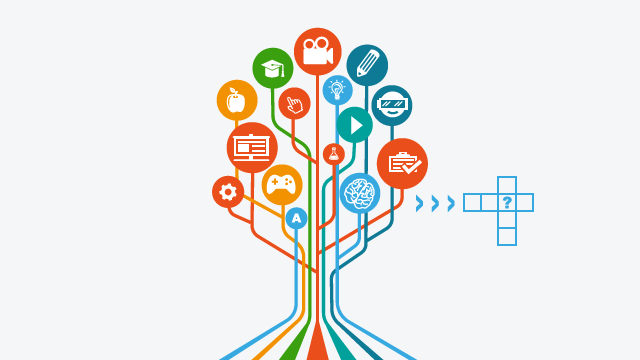
\includegraphics[scale=0.5]{images/arvore.png}
	\caption{Conceito Objeto de Aprendizado}
	\label{img:arvore}
\end{figure}
Figura \ref{img:arvore} representa como os objetos podem ser exportados para o aprendizado.

\begin{figure}[htb]
	\centering
	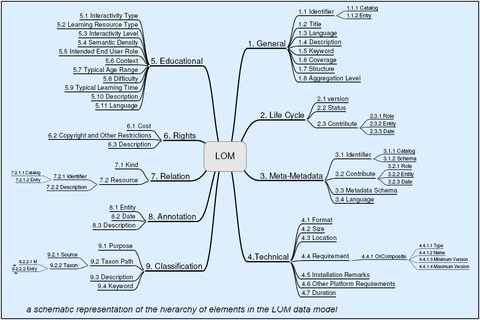
\includegraphics[scale=1.0]{images/lom.png}
	\caption{Metadados de objetos de aprendizado}
	\label{img:lom}
\end{figure}
Figura \ref{img:lom} demonstra uma especificação de metadados para objetos de aprendizado.

\cleardoublepage

\postextual

%%Colocar as referências conforme as normas da ABNT, somente as utilizadas no trabalho e presentes neste manuscrito.

\begin{thebibliography}{99}

\bibitem{LTSC:2002}
{IEEE Learning Technology Standards Committee (LTSC) available at: IEEE 1484.12.1-2002, 15 July 2002, \textbf{Draft Standard for Learning Object Metadata.}}

\bibitem{Sathiyamurthy:2012}
{K. Sathiyamurthy, T. V. Geetha, and M. Senthilvelan. 2012. \textbf{An approach towards dynamic assembling of learning objects.} In Proceedings of the International Conference on Advances in Computing, Communications and Informatics (ICACCI '12), Sabu M. Thampi, El-Sayed El-Afry, and Javier Aguiar (Eds.). ACM, New York, NY, USA, 1193-1198.}

\bibitem{McGreal:2004}
{MCGREAL, R. \textbf{Learning objects: A practical definition} International Journal of Instructional Technology and Distance Learning (IJITDL).2004/9/4}

\bibitem{Braga:2012}
{Braga J, Dotta S, Pimentel E, Stransky B (2012) \textbf{Desafios para o
Desenvolvimento de Objetos de Aprendizagem Reutilizáveis e de Qualidade.} In: Anais do Workshop de Desafios da Computação Aplicada à Educação., pp 90-99.}

\bibitem{Downes:2003}
{Downes, S. (2003). \textbf{Design and reusability of learning objects in an academic context: A new economy of education?} Journal of the United States Distance Learning Association, 17(1).}

\bibitem{Degen:2001}
{Degen, B. (2001). \textbf{Capitalizing on the learning object economy: The strategic benefits of standard learning objects.} Learning Objects Network, Inc.}

\bibitem{Bannan:2002}
{Bannan-Ritland, B., Dabbagh, N., Murphy, K. (2002). \textbf{Learning object systems as constructivist learning environments: Related assumptions, theories and applications.} In D.A. Wiley (Ed.), The instructional
use of learning objects. Bloomington, IN.}

\bibitem{Siegmund:2014}
{Janet Siegmund, Christian Kästner, Sven Apel, Chris Parnin, Anja Bethmann, Thomas Leich, Gunter Saake, and André Brechmann. 2014. \textbf{Understanding understanding source code with functional magnetic resonance imaging.} In Proceedings of the 36th International Conference on Software Engineering (ICSE 2014). ACM, New York, NY, USA, 378-389.}

\bibitem{Framin:2013}
{Andrés Framiñán, Pablo Ruisoto, Diana García, and Juan A. Juanes. 2013. \textbf{Advanced neuroimage processing for the study of the neurovascular system.} In Proceedings of the First International Conference on Technological Ecosystem for Enhancing Multiculturality (TEEM '13), Francisco José García-Peñalvo (Ed.). ACM, New York, NY, USA, 37-41.}

\bibitem{Polsani:2003} 
{olsani, P. R. (2003). \textbf{Use and abuse of reusable learning objects.} Journal of Digital Information, 3(4).}

\bibitem{Longmire:2001}
{Longmire, W. (2001). \textbf{A primer on learning objects.} Learning Circuits. Dísponivel em: http://kennison.name/files/learning/learning-object-design.pdf. Acesso em: 09 out 2017.}

\end{thebibliography}

\end{document}